\documentclass[aspectratio=169,10pt]{beamer}

\usepackage{fontspec}
\usepackage{polyglossia}
\setdefaultlanguage{english}
\setotherlanguage{vietnamese}
\setmainfont{DejaVu Sans}
\setsansfont{DejaVu Sans}
\setmonofont{DejaVu Sans Mono}

\usepackage{tikz}
\usetikzlibrary{arrows.meta,positioning,shapes.geometric,fit,calc}
\usepackage{xcolor}
\usepackage{listings}
\usepackage{booktabs}
\usepackage{array}

\usetheme{Madrid}
\usecolortheme{seahorse}
\setbeamertemplate{navigation symbols}{}
\newcommand{\TotalFramesFixed}{49}
\setbeamertemplate{footline}{%
  \leavevmode%
  \hbox{\begin{beamercolorbox}[wd=\paperwidth,ht=2.6ex,dp=1.1ex,right]{page number in head/foot}%
    \usebeamerfont{page number in head/foot}\insertframenumber/\TotalFramesFixed\hspace*{1.5ex}
  \end{beamercolorbox}}%
}

\definecolor{pyblue}{HTML}{1F77B4}
\definecolor{pygreen}{HTML}{2CA02C}
\definecolor{pyorange}{HTML}{FF7F0E}
\definecolor{pypurple}{HTML}{9467BD}
\definecolor{pygray}{HTML}{F2F4F8}
\definecolor{dark}{HTML}{1F2937}

\lstdefinestyle{pythonstyle}{
  language=Python,
  basicstyle=\ttfamily\small,
  keywordstyle=\color{pyblue}\bfseries,
  commentstyle=\color{pygreen},
  stringstyle=\color{pyorange},
  showstringspaces=false,
  columns=fullflexible,
  keepspaces=true,
  frame=single,
  rulecolor=\color{gray!40},
  backgroundcolor=\color{pygray},
  breaklines=true
}
\lstset{style=pythonstyle}

\tikzset{
  box/.style={draw=dark, rounded corners=2mm, very thick, align=center, fill=pygray, minimum height=10mm, inner sep=2.5mm},
  bluebox/.style={box, fill=blue!12},
  greenbox/.style={box, fill=green!12},
  orangebox/.style={box, fill=orange!16},
  purplebox/.style={box, fill=purple!12},
  arrow/.style={-{Latex[length=2.5mm]}, very thick, draw=dark}
}

\title[Lesson 1: Introduction]{Lesson 1. Introduction: Computers, Python, and Algorithms}
\subtitle{Based on Chapter 1 -- Python for Everyone, 3rd Edition}
\author{Course: Introduction to Python Programming}
\date{}

\begin{document}

\begin{frame}[plain]
\vspace{0.4cm}
\begin{columns}[T,onlytextwidth]
\column{0.62\textwidth}
{\LARGE\bfseries Lesson 1. Introduction:\\[0.12cm] Computers, Python, and Algorithms\par}
\vspace{0.35cm}
{\large Based on Chapter 1 -- \textit{Python for Everyone}, 3rd Edition\par}
\vspace{0.45cm}
\begin{block}{Lecture information}
\small
\begin{itemize}
  \item Course: Introduction to Python Programming
  \item Topics: computer programs, computer components, Python, common errors, algorithms
  \item Main reference: Cay Horstmann and Rance Necaise
\end{itemize}
\end{block}

\column{0.34\textwidth}
\begin{center}
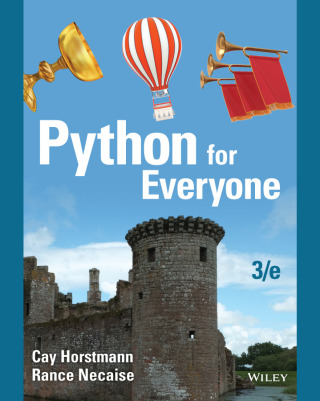
\includegraphics[width=0.9\linewidth,height=0.58\paperheight,keepaspectratio]{horstmann_book_cover_page1.png}\\[0.15cm]
{\scriptsize Book cover used as a source reference}
\end{center}
\end{columns}
\vfill
\hfill {\scriptsize 1/49}
\end{frame}

\begin{frame}{Learning objectives}
After this lesson, students will be able to:
\begin{itemize}
  \item explain computer programs and programming;
  \item describe the basic components of a computer;
  \item run their first Python program;
  \item analyze the \texttt{Hello, World!} program;
  \item distinguish compile-time errors, exceptions, and logic errors;
  \item describe algorithms using pseudocode.
\end{itemize}
\end{frame}

\begin{frame}{Chapter 1 structure}
\begin{enumerate}
  \item Computer Programs
  \item The Anatomy of a Computer
  \item The Python Programming Language
  \item Programming Environment
  \item First Python Program
  \item Errors
  \item Algorithm Design and Pseudocode
\end{enumerate}
\end{frame}

\section{Computer Programs}

\begin{frame}{Computers and programs}
\begin{block}{Computer program}
A computer program is a sequence of \textbf{instructions} and \textbf{decisions} that asks the computer to perform a specific task.
\end{block}
\begin{center}
\begin{tikzpicture}[scale=0.88, every node/.style={transform shape}]
  \node[greenbox, minimum width=3.2cm] (program) at (0,0) {Program\\instructions + decisions};
  \node[orangebox, minimum width=3.0cm] (computer) at (4.9,0) {Computer\\executes};
  \node[purplebox, minimum width=2.9cm] (result) at (9.4,0) {Result\\output};
  \draw[arrow] (program.east) -- (computer.west);
  \draw[arrow] (computer.east) -- (result.west);
  \node[box, align=left, minimum width=10.2cm] (task) at (4.7,-2.1) {\textbf{Example task:} ask the user for a name, print a greeting,\\and optionally print a welcome message.};
\end{tikzpicture}
\end{center}
\begin{alertblock}{Key idea}
The same computer can perform many different tasks because it can run many different programs.
\end{alertblock}
\end{frame}

\begin{frame}{What is programming?}
\begin{block}{Programming}
Programming is the act of \textbf{designing} and \textbf{implementing} computer programs.
\end{block}

\begin{center}
\begin{tikzpicture}[scale=0.92, every node/.style={transform shape}]
  \node[bluebox, minimum width=2.3cm] (problem) at (0,0) {Problem\\to solve};
  \node[greenbox, minimum width=2.5cm] (steps) at (3.2,0) {Clear\\steps};
  \node[orangebox, minimum width=2.3cm] (code) at (6.5,0) {Python\\code};
  \node[purplebox, minimum width=2.5cm] (run) at (9.8,0) {Computer\\executes};
  \node[bluebox, minimum width=2.5cm] (output) at (13.0,0) {Output\\result};
  \draw[arrow] (problem) -- (steps);
  \draw[arrow] (steps) -- (code);
  \draw[arrow] (code) -- (run);
  \draw[arrow] (run) -- (output);
  \draw[arrow, dashed] (output.south) .. controls +(0,-1.0) and +(0,-1.0) .. node[below]{check and fix} (code.south);
\end{tikzpicture}
\end{center}

\vspace{0.1cm}
\begin{itemize}
  \item A computer does not guess intentions; it follows instructions.
  \item The programmer translates a problem into executable steps.
\end{itemize}
\end{frame}

\begin{frame}{Hardware and Software}
\begin{center}
\begin{tikzpicture}[scale=0.86, every node/.style={transform shape}]
  \node[bluebox, minimum width=4.7cm, minimum height=1.25cm] (user) at (-0.3,2.9) {User};
  \node[greenbox, minimum width=4.7cm, minimum height=1.35cm] (apps) at (-0.3,0.9) {Application Software\\browser, apps, games};
  \node[orangebox, minimum width=4.7cm, minimum height=1.25cm] (os) at (-0.3,-1.2) {Operating System\\Windows, Linux, macOS};
  \node[purplebox, minimum width=4.7cm, minimum height=1.25cm] (hw) at (-0.3,-3.3) {Hardware\\CPU, RAM, disk, screen};

  \draw[arrow] (user.south) -- (apps.north);
  \draw[arrow] (apps.south) -- (os.north);
  \draw[arrow] (os.south) -- (hw.north);

  \node[box, align=left, text width=6.8cm] (note) at (7.8,-0.6) {\textbf{Key idea}\\
Software describes what to do.\\
Hardware performs physical operations.\\
The OS manages resources as an intermediate layer.};

  % simple 90-degree bent dashed arrow showing results/data returning to application software
  \draw[arrow, dashed] (hw.east) -- ++(1.1,0) -- ++(0,3.0) -- (apps.east);
  \node[align=center] at (3.35,-0.15) {data and\\results};
\end{tikzpicture}
\end{center}
\end{frame}

\begin{frame}{Self Check 1}
\begin{enumerate}
  \item A computer program is a sequence of \underline{\hspace{2cm}} and decisions.
  \item Programming is the process of designing and implementing computer programs. True or false?
  \item Why can the same computer perform many different kinds of tasks?
\end{enumerate}
\end{frame}

\begin{frame}{Answers to Self Check 1}
\begin{enumerate}
  \item Instructions.
  \item True.
  \item Because the hardware can run many different programs; each program describes a specific task.
\end{enumerate}
\end{frame}

\section{The Anatomy of a Computer}

\begin{frame}{Main components of a computer}
\begin{center}
\begin{tikzpicture}[scale=0.85, every node/.style={transform shape}]
  \node[bluebox, minimum width=2.5cm] (input) at (0,0) {Input\\keyboard, mouse\\camera, mic};
  \node[greenbox, minimum width=2.7cm] (cpu) at (4,0) {CPU\\program control\\data processing};
  \node[orangebox, minimum width=2.7cm] (mem) at (4,2.1) {Memory\\running data\\programs};
  \node[purplebox, minimum width=2.7cm] (disk) at (4,-2.1) {Secondary\\Storage\\SSD/HDD};
  \node[bluebox, minimum width=2.5cm] (out) at (8,0) {Output\\monitor, printer\\speakers};
  \node[greenbox, minimum width=2.5cm] (net) at (8,-2.1) {Network\\Internet};
  \draw[arrow] (input) -- (cpu);
  \draw[arrow] (cpu) -- (out);
  \draw[arrow] (cpu) -- (mem);
  \draw[arrow] (mem) -- (cpu);
  \draw[arrow] (cpu) -- (disk);
  \draw[arrow] (disk) -- (cpu);
  \draw[arrow] (cpu) -- (net);
  \draw[arrow] (net) -- (cpu);
\end{tikzpicture}
\end{center}
\end{frame}

\begin{frame}[plain]
\centering
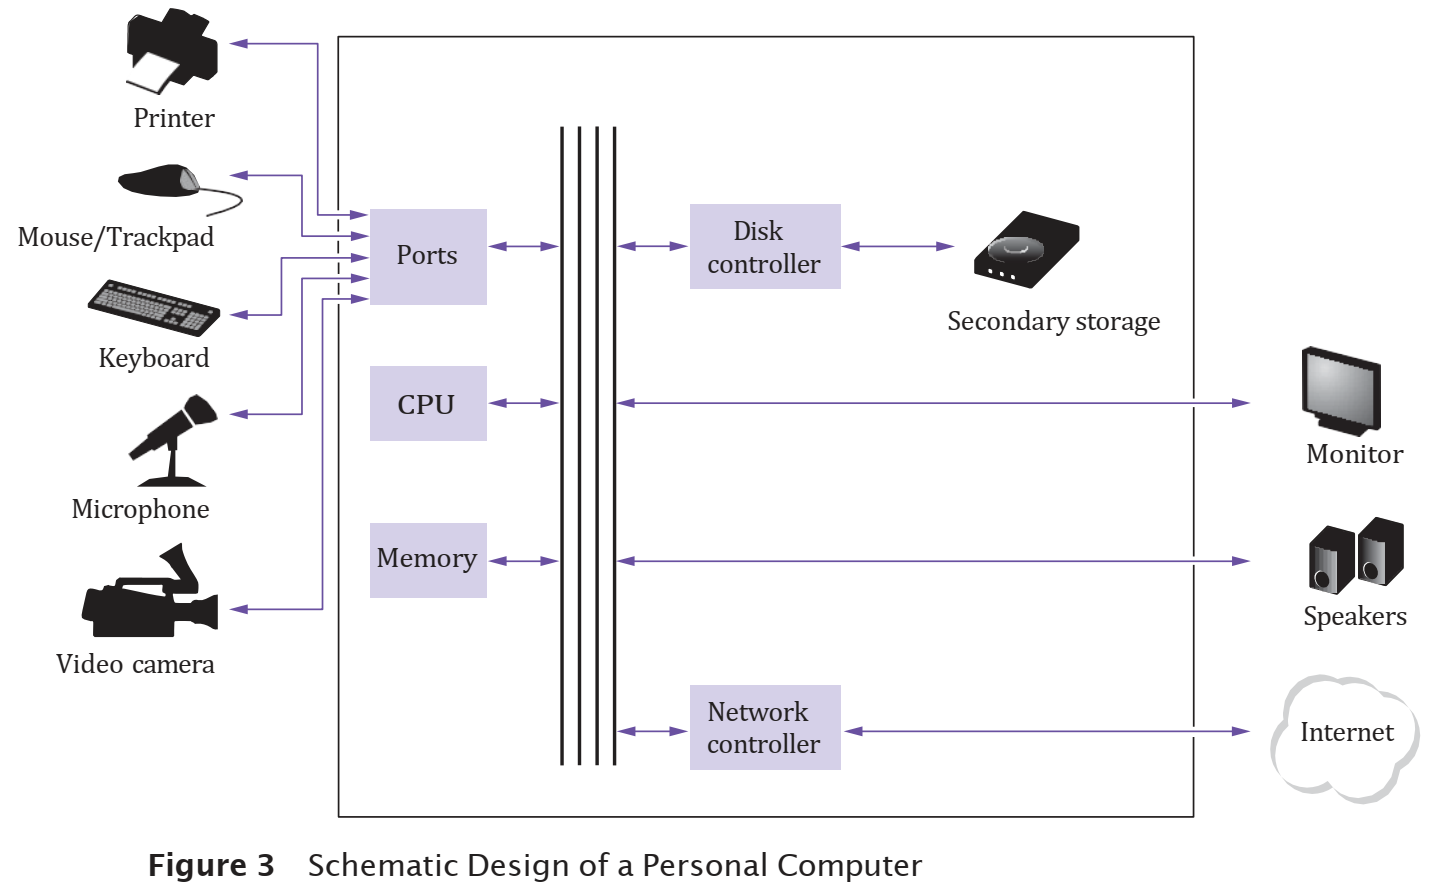
\includegraphics[width=\paperwidth,height=0.92\paperheight,keepaspectratio]{insert_after_page9_what_does_computer_do.png}
\end{frame}

\begin{frame}{CPU, memory, and storage}
\begin{description}
  \item[CPU] Controls programs and processes data.
  \item[Memory] Stores programs and data currently in use; fast but usually not persistent after power-off.
  \item[Secondary storage] Provides long-term storage, such as hard drives, SSDs, and USB drives.
\end{description}

\vspace{0.3cm}
\begin{alertblock}{Key idea}
When a program runs, its file is usually speakersded from secondary storage into memory so the CPU can read and execute it.
\end{alertblock}
\end{frame}

\begin{frame}{Input, output, and network}
\small
\begin{columns}[T,onlytextwidth]
\column{0.31\textwidth}
\begin{block}{Input}
Data enters the computer.
\begin{itemize}
  \item keyboard
  \item mouse
  \item microphone
  \item camera
\end{itemize}
\end{block}

\column{0.31\textwidth}
\begin{block}{Output}
Information produced by the computer.
\begin{itemize}
  \item monitor
  \item speakers
  \item printer
\end{itemize}
\end{block}

\column{0.31\textwidth}
\begin{block}{Network}
Exchanges data with\\
other computers.
\begin{itemize}
  \item local network
  \item Internet
  \item remote server
\end{itemize}
\end{block}
\end{columns}
\end{frame}

\begin{frame}{Computers Are Everywhere}
Computers are not only laptops or PCs.
\begin{itemize}
  \item Smartphones, bank cards, and transit cards.
  \item Modern cars, medical devices, factories, and robots.
  \item Data centers, social networks, and e-commerce.
\end{itemize}

\begin{block}{Message}
\small Understanding computers and programming helps students work better\\
in many fields, not only information technology.
\end{block}
\end{frame}

\begin{frame}{Self Check 2}
\begin{enumerate}
  \item Which component controls programs and processes data?
  \item Secondary storage usually keeps data after power-off. True or false?
  \item Keyboard and mouse belong to which device group?
\end{enumerate}
\end{frame}

\begin{frame}{Answers to Self Check 2}
\begin{enumerate}
  \item CPU.
  \item True.
  \item Input devices.
\end{enumerate}
\end{frame}

\section{Python Programming Language}

\begin{frame}[fragile]{Python is a high-level programming language}
\small
\begin{columns}[T,onlytextwidth]
\column{0.57\textwidth}
\begin{block}{High-level language}
A language close to how humans describe problems; easier to read and write.

\textbf{Examples:} Python, Java, C++, JavaScript.

\textbf{High-level command example:} \texttt{print("Hello, World!")}
\end{block}

\vspace{0.18cm}
\begin{block}{Low-level language}
A language closer to hardware and the CPU; harder to read but gives more detailed machine control.

\textbf{Examples:} machine code, assembly language.

\textbf{Low-level command example:} \texttt{MOV AX, 1}
\end{block}

\column{0.37\textwidth}
\begin{center}
\begin{tikzpicture}[scale=0.60, every node/.style={transform shape}]
  \node[bluebox, minimum width=4.0cm, minimum height=1.05cm] (idea) at (0,3.6) {Human\\idea};
  \node[greenbox, minimum width=4.0cm, minimum height=1.15cm] (high) at (0,1.5) {High-level\\Python code};
  \node[orangebox, minimum width=4.0cm, minimum height=1.15cm] (inter) at (0,-0.8) {Interpreter\\translates/executes};
  \node[purplebox, minimum width=4.0cm, minimum height=1.15cm] (low) at (0,-3.1) {Low-level\\machine/assembly};
  \node[bluebox, minimum width=4.0cm, minimum height=1.05cm] (cpu) at (0,-5.3) {CPU\\executes instructions};
  \draw[arrow] (idea.south) -- (high.north);
  \draw[arrow] (high.south) -- (inter.north);
  \draw[arrow] (inter.south) -- (low.north);
  \draw[arrow] (low.south) -- (cpu.north);
\end{tikzpicture}
\end{center}
\end{columns}
\end{frame}

\begin{frame}{Packages in Python}
\begin{block}{Package}
A package provides ready-made code for a specific problem domain.
\end{block}
\begin{center}
\begin{tikzpicture}[scale=0.94, every node/.style={transform shape}]
  \node[bluebox, minimum width=1.9cm] (py) at (0,0) {Python};
  \node[greenbox, minimum width=3.1cm] (ds) at (-4.7,-2.1) {Data Science};
  \node[greenbox, minimum width=4.0cm] (ml) at (0,-2.1) {Machine Learning};
  \node[greenbox, minimum width=3.2cm] (viz) at (4.7,-2.1) {Visualization};
  \node[orangebox, minimum width=8.3cm] (reuse) at (0,-4.65) {Reuse existing code\\reduce effort from writing from scratch};
  \draw[arrow] (py.south west) -- (ds.north east);
  \draw[arrow] (py.south) -- (ml.north);
  \draw[arrow] (py.south east) -- (viz.north west);
  % centered vertical arrows from each concept block to the reuse block
  \draw[arrow] (ds.south) -- ([xshift=-3.2cm]reuse.north);
  \draw[arrow] (ml.south) -- (reuse.north);
  \draw[arrow] (viz.south) -- ([xshift=3.2cm]reuse.north);
\end{tikzpicture}
\end{center}
\end{frame}

\begin{frame}{Self Check 3}
\begin{enumerate}
  \item Is Python a high-level or low-level programming language?
  \item Python can run on only one operating system. True or false?
  \item How do packages help programmers?
\end{enumerate}
\end{frame}

\begin{frame}{Answers to Self Check 3}
\begin{enumerate}
  \item High-level.
  \item False.
  \item Packages provide ready-made code for different problem domains and help reuse existing solutions.
\end{enumerate}
\end{frame}

\section{Programming Environment}

\begin{frame}{Getting familiar with the programming environment}
A programming environment usually includes:
\begin{itemize}
  \item Python interpreter;
  \item a text editor or IDE;
  \item terminal/command prompt;
  \item a folder for storing program files;
  \item tools for running and testing programs.
\end{itemize}

\begin{alertblock}{Note}
Students should spend time getting familiar with the tools before working on larger assignments.
\end{alertblock}
\end{frame}

\begin{frame}[fragile]{The first program}
Create the file \texttt{hello.py}:

\begin{lstlisting}
# My first Python program.
print("Hello, World!")
\end{lstlisting}

Expected output:

\begin{lstlisting}
Hello, World!
\end{lstlisting}

\begin{itemize}
  \item Python is case-sensitive.
  \item \texttt{print} is different from \texttt{Print}.
\end{itemize}
\end{frame}

\begin{frame}{Organizing the working folder}
\begin{center}
\begin{tikzpicture}[node distance=0.65cm]
  \node[box, align=left, minimum width=7.2cm] (root) {python-course/};
  \node[box, align=left, below=of root, xshift=-1.4cm, minimum width=4.0cm] (ch1) {chapter01/\\\quad hello.py\\\quad exercises/};
  \node[box, align=left, below=of root, xshift=2.6cm, minimum width=4.0cm] (ch2) {chapter02/\\\quad notes/};
  \draw[arrow] (root.south) -- (ch1.north);
  \draw[arrow] (root.south) -- (ch2.north);
\end{tikzpicture}
\end{center}

\begin{itemize}
  \item Python files usually have the \texttt{.py} extension.
  \item It is useful to have a separate folder for each chapter/assignment.
  \item A backup strategy is needed.
\end{itemize}
\end{frame}

\begin{frame}[fragile]{Interactive Mode}
Interactive mode lets you run commands one by one and immediately see the results.

\begin{lstlisting}
>>> print("Hello, World!")
Hello, World!
>>> 7035 * 0.15
1055.25
\end{lstlisting}

\begin{itemize}
  \item Quickly test expressions.
  \item Check new syntax.
  \item Use Python as a pocket calculator.
\end{itemize}
\end{frame}

\begin{frame}{From source code to running program}
\begin{center}
\begin{tikzpicture}[scale=0.93, every node/.style={transform shape}]
  \node[bluebox, minimum width=1.45cm] (editor) at (0,0) {Editor};
  \node[greenbox, minimum width=2.2cm] (source) at (2.6,0) {Source File\\\texttt{.py}};
  \node[orangebox, minimum width=1.95cm] (compiler) at (5.25,0) {Compiler};
  \node[purplebox, minimum width=2.0cm] (bytecode) at (7.95,0) {Byte Code};
  \node[greenbox, minimum width=2.05cm] (vm) at (10.75,0) {Virtual\\Machine};
  \node[bluebox, minimum width=2.2cm] (run) at (13.55,0) {Running\\Program};
  \node[box, minimum width=2.2cm] (stdlib) at (9.25,-2.95) {Standard\\Library};
  \node[box, minimum width=2.55cm] (pkg) at (12.05,-2.95) {Additional\\Packages};
  \draw[arrow] (editor) -- (source);
  \draw[arrow] (source) -- (compiler);
  \draw[arrow] (compiler) -- (bytecode);
  \draw[arrow] (bytecode) -- (vm);
  \draw[arrow] (vm) -- (run);
  \draw[arrow] (stdlib.north) -- (vm.south);
  \draw[arrow] (pkg.north) -- (vm.south);
\end{tikzpicture}
\end{center}
\end{frame}

\begin{frame}{Self Check 4}
\begin{enumerate}
  \item What extension do Python program files usually have?
  \item Is Python case-sensitive?
  \item What is the tool that reads and executes Python programs called?
\end{enumerate}
\end{frame}

\begin{frame}{Answers to Self Check 4}
\begin{enumerate}
  \item \texttt{.py}
  \item Yes.
  \item Python interpreter.
\end{enumerate}
\end{frame}

\section{Analyzing Your First Program}

\begin{frame}[fragile]{Analyzing the first program}
\begin{lstlisting}
# My first Python program.
print("Hello, World!")
\end{lstlisting}

\begin{description}
  \item[Comment] starts with \texttt{\#} and is used to explain code to readers.
  \item[Statement] a command that asks Python to perform an action.
  \item[Function] \texttt{print} is a built-in function.
  \item[Argument] \texttt{"Hello, World!"} is the value passed to the function.
  \item[String] a sequence of characters enclosed in quotation marks.
\end{description}
\end{frame}

\begin{frame}[fragile]{Strings and expressions}
Compare these two statements:

\begin{lstlisting}
print("39 + 3")
print(39 + 3)
\end{lstlisting}

Output:

\begin{lstlisting}
39 + 3
42
\end{lstlisting}

\begin{itemize}
  \item The first line prints the literal string.
  \item The second line evaluates the expression and prints the result.
\end{itemize}
\end{frame}

\begin{frame}[fragile]{The print syntax}
\begin{lstlisting}
print(value1, value2, ..., valuen)
\end{lstlisting}

Example:

\begin{lstlisting}
print("The answer is", 6 + 7, "!")
\end{lstlisting}

\begin{itemize}
  \item Values are printed in order.
  \item By default, they are separated by spaces.
  \item \texttt{print()} with no arguments prints a blank line.
\end{itemize}
\end{frame}

\begin{frame}{Self Check 5}
\begin{enumerate}
  \item What character begins a Python comment?
  \item What is a value passed to a function called?
  \item How are \texttt{print("39 + 3")} and \texttt{print(39 + 3)} different?
\end{enumerate}
\end{frame}

\begin{frame}{Answers to Self Check 5}
\begin{enumerate}
  \item The \texttt{\#} character.
  \item Argument.
  \item The first statement prints the string \texttt{39 + 3}; the second evaluates the addition and prints \texttt{42}.
\end{enumerate}
\end{frame}

\section{Errors}

\begin{frame}{Three common groups of errors}
\begin{center}
\begin{tikzpicture}[scale=0.93, every node/.style={transform shape}]
  % top process row
  \node[bluebox, minimum width=2.4cm] (write) at (0,0) {Write code};
  \node[greenbox, minimum width=3.2cm] (compile) at (3.9,0) {Translate / check\\syntax};
  \node[orangebox, minimum width=2.9cm] (run) at (8.1,0) {Run program};
  \node[purplebox, minimum width=2.8cm] (observe) at (12.0,0) {Observe\\result};

  % horizontal process arrows
  \draw[arrow] (write.east) -- (compile.west);
  \draw[arrow] (compile.east) -- (run.west);
  \draw[arrow] (run.east) -- (observe.west);

  % error blocks placed lower with more spacing
  \node[bluebox, minimum width=3.3cm] (syntax) at (3.9,-2.4) {Syntax error\\before running};
  \node[orangebox, minimum width=3.1cm] (exception) at (8.1,-2.4) {Exception\\while running};
  \node[purplebox, minimum width=3.3cm] (logic) at (12.0,-2.4) {Logic error\\wrong result};

  % vertical arrows from stages to corresponding errors
  \draw[-{Latex[length=2.4mm]}, thick, draw=dark, dashed] (compile.south) -- (syntax.north);
  \draw[-{Latex[length=2.4mm]}, thick, draw=dark, dashed] (run.south) -- (exception.north);
  \draw[-{Latex[length=2.4mm]}, thick, draw=dark, dashed] (observe.south) -- (logic.north);
\end{tikzpicture}
\end{center}

\vspace{0.2cm}
\begin{itemize}
  \item The location of an error helps us know how to inspect and fix the program.
\end{itemize}
\end{frame}

\begin{frame}[fragile]{Examples of errors}
\small
\begin{columns}[T,onlytextwidth]
\column{0.315\textwidth}
\begin{block}{Syntax error}
\begin{lstlisting}
print("Hello)
\end{lstlisting}
Missing quotation mark.
\end{block}

\column{0.315\textwidth}
\begin{block}{Exception}
\begin{lstlisting}
print(1 / 0)
\end{lstlisting}
Division by zero.
\end{block}

\column{0.315\textwidth}
\begin{block}{Logic error}
\begin{lstlisting}
print("Hello, Word!")
\end{lstlisting}
Runs, but does not match the intended result.
\end{block}
\end{columns}
\end{frame}

\begin{frame}[fragile]{Common Error: Misspelling Words}
\begin{lstlisting}
Print("Hello, World!")
\end{lstlisting}

\begin{itemize}
  \item Python case sensitive.
  \item \texttt{Print} is not the same as \texttt{print}.
  \item When an error is hard to understand, check spelling and capitalization.
\end{itemize}
\end{frame}

\begin{frame}{Self Check 6}
\begin{enumerate}
  \item What is an error that violates syntax rules called?
  \item What is an error that occurs when a syntactically correct statement cannot be executed?
  \item Are \texttt{Print} and \texttt{print} the same in Python?
\end{enumerate}
\end{frame}

\begin{frame}{Answers to Self Check 6}
\begin{enumerate}
  \item A compile-time error or syntax error.
  \item Exception.
  \item No. Python is case-sensitive.
\end{enumerate}
\end{frame}

\section{Algorithm Design}

\begin{frame}{Problem-solving thinking}
\begin{block}{Before writing code}
Understand the problem and describe the solution with clear steps.
\end{block}
\begin{center}
\begin{tikzpicture}[scale=0.9, every node/.style={transform shape}]
  \node[bluebox, minimum width=2.8cm] (messy) at (0,0) {Real-world problem\\unclear description};
  \node[greenbox, minimum width=2.8cm] (inputs) at (3.5,1.1) {Identify\\input/output};
  \node[greenbox, minimum width=2.8cm] (steps) at (3.5,-1.1) {Break into\\small steps};
  \node[orangebox, minimum width=2.8cm] (algo) at (7.0,0) {Clear\\algorithm};
  \node[purplebox, minimum width=2.8cm] (code) at (10.5,0) {Python\\program};
  \draw[arrow] (messy) -- (inputs);
  \draw[arrow] (messy) -- (steps);
  \draw[arrow] (inputs) -- (algo);
  \draw[arrow] (steps) -- (algo);
  \draw[arrow] (algo) -- (code);
\end{tikzpicture}
\end{center}
\end{frame}

\begin{frame}{Algorithm and pseudocode}
\begin{columns}[T]
\column{0.48\textwidth}
\begin{block}{Algorithm}
A sequence of steps for solving a problem; it should be:
\begin{itemize}
  \item unambiguous;
  \item executable;
  \item terminating.
\end{itemize}
\end{block}
\begin{block}{Pseudocode}
A human-readable description of an algorithm before translating it into code.
\end{block}

\column{0.48\textwidth}
\begin{center}
\begin{tikzpicture}[scale=0.8, every node/.style={transform shape}]
  \node[greenbox, minimum width=3.8cm] (u) at (0,1.8) {Unambiguous\\unambiguous};
  \node[orangebox, minimum width=3.8cm] (e) at (0,0) {Executable\\executable};
  \node[purplebox, minimum width=3.8cm] (t) at (0,-1.8) {Terminating\\terminating};
  \node[bluebox, minimum width=3.8cm] (a) at (4.1,0) {Algorithm};
  \draw[arrow] (u.east) -- (a.north west);
  \draw[arrow] (e.east) -- (a.west);
  \draw[arrow] (t.east) -- (a.south west);
\end{tikzpicture}
\end{center}
\end{columns}
\end{frame}

\begin{frame}[fragile]{Pseudocode example: bank account}
Problem: deposit 10,000 USD with 5\% annual interest. How many years until the balance at least doubles?

\begin{lstlisting}[language={}]
Set year to 0
Set balance to 10000
While balance is less than 20000
    Add 1 to year
    Set interest to balance x 0.05
    Add interest to balance
Report year as the answer
\end{lstlisting}
\end{frame}

\begin{frame}{A simple software development process}
\begin{center}
\begin{tikzpicture}[node distance=0.85cm]
  \node[bluebox] (p) {Understand\\the problem};
  \node[greenbox, right=of p] (a) {Develop\\algorithm};
  \node[orangebox, right=of a] (t) {Test with\\simple inputs};
  \node[purplebox, right=of t] (py) {Translate\\to Python};
  \node[bluebox, right=of py] (ct) {Compile\\and test};
  \draw[arrow] (p) -- (a);
  \draw[arrow] (a) -- (t);
  \draw[arrow] (t) -- (py);
  \draw[arrow] (py) -- (ct);
\end{tikzpicture}
\end{center}
\end{frame}

\begin{frame}{Data Is Everywhere}
\begin{center}
\begin{tikzpicture}[scale=0.88, every node/.style={transform shape}]
  \node[bluebox, minimum width=2.6cm] (collect) at (0,0) {Collect\\data};
  \node[greenbox, minimum width=2.8cm] (clean) at (3.1,0) {Clean and\\organize};
  \node[orangebox, minimum width=2.8cm] (analyze) at (6.4,0) {Analyze /\\model};
  \node[purplebox, minimum width=2.8cm] (decision) at (9.8,0) {Predict /\\decide};
  \draw[arrow] (collect) -- (clean);
  \draw[arrow] (clean) -- (analyze);
  \draw[arrow] (analyze) -- (decision);
  \node[box, align=left, minimum width=9.8cm] (examples) at (4.9,-2.2) {\textbf{Examples:} customer analytics, fraud detection, image recognition,\\medical diagnosis support, self-driving cars.};
\end{tikzpicture}
\end{center}
\end{frame}

\begin{frame}[fragile]{How To: write pseudocode}
Problem: choose which car is more economical over 10 years.

\begin{lstlisting}[language={}]
For each car, compute total cost:
    annual fuel consumed = annual miles driven / fuel efficiency
    annual fuel cost = price per gallon x annual fuel consumed
    operating cost = 10 x annual fuel cost
    total cost = purchase price + operating cost

If total cost of car 1 < total cost of car 2
    Choose car 1
Else
    Choose car 2
\end{lstlisting}
\end{frame}

\begin{frame}[fragile]{Worked Example: tiling a floor}
Problem: tile a floor with alternating black and white tiles, each \(4 \times 4\) inches.

\begin{lstlisting}[language={}]
Place a black tile in the northwest corner
While the floor is not yet filled
    Repeat width / 4 - 1 times
        If previous tile was white
            Pick a black tile
        Else
            Pick a white tile
        Place the picked tile east of previous tile
    If there is space to the south
        Place opposite color below first tile of row
\end{lstlisting}
\end{frame}

\begin{frame}{Self Check 7}
\begin{enumerate}
  \item What is pseudocode?
  \item What three properties should an algorithm have?
  \item Why should we test an algorithm with small examples before writing code?
\end{enumerate}
\end{frame}

\begin{frame}{Answers to Self Check 7}
\begin{enumerate}
  \item An informal description of the steps for solving a problem.
  \item Unambiguous, executable, and terminating.
  \item To detect errors in the idea before translating it into Python.
\end{enumerate}
\end{frame}

\section{Practice}

\begin{frame}{In-class practice exercises}
\begin{enumerate}
  \item Create \texttt{hello.py} and run the \texttt{Hello, World!} program.
  \item Create a syntax error, read the error message, and fix it.
  \item Compare \texttt{print("39 + 3")} and \texttt{print(39 + 3)}.
  \item Open interactive mode and run a few arithmetic expressions.
  \item Write pseudocode for splitting a restaurant bill.
\end{enumerate}
\end{frame}

\begin{frame}{Quick quiz}
\begin{enumerate}
  \item What extension do Python files usually have?
  \item Is \texttt{print} a function or a string?
  \item What symbols enclose a string?
  \item What error usually occurs when dividing by zero while running?
  \item Does pseudocode have to follow Python syntax exactly?
\end{enumerate}
\end{frame}

\begin{frame}{Answers to Quick quiz}
\begin{enumerate}
  \item \texttt{.py}
  \item Function.
  \item Single or double quotation marks.
  \item Exception.
  \item No.
\end{enumerate}
\end{frame}

\begin{frame}{Summary}
\begin{itemize}
  \item Program = instructions + decisions.
  \item CPU, memory, storage, input/output, and network components work together to run programs.
  \item Python is easy to learn, portable, and has many packages.
  \item The first program helps explain comments, functions, arguments, and strings.
  \item Errors are normal; we need to know how to read and classify them.
  \item Before coding, understand the problem and write the algorithm in pseudocode.
\end{itemize}
\end{frame}

\end{document}
